\section{Газовые законы}

\begin{wrapfigure}{r}{3cm}
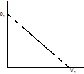
\includegraphics{082001GasLawsProcess.jpg}
\end{wrapfigure}

%1
\AddProb (2001) Какой максимальной температуры достигнет газ в процессе, изображенном на рисунке? Показатель адиабаты $\gamma$ считать известным.

\AddProb (2010) Посередине откаченной и запаянной с обоих концов горизонтально расположенной трубки длины $L$ находится столбик ртути длины $h$. 
Если трубку поставить вертикально, столбик ртути смеситься на расстояние $x$. Какое первоначальное давление в трубке? Плотность ртути $\rho$.

\AddProb (2013) В баллон, вместимостью $V$, при давлении $p$ нагнетают воздух. 
За какое время $t$ он будет накачан до давления $p_n$, если компрессор за время $\tau$ засасывает объем $V_0$ атмосферного воздуха? 
Температуру считать неизменной, а атмосферное давление равным $p_0$. Как изменится ответ, если воздух откачивать из баллона?

\begin{wrapfigure}{r}{3.5cm}
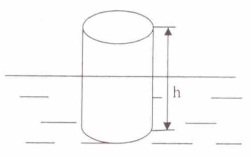
\includegraphics[scale=0.5]{082012GasLawsGlass.jpg}
\end{wrapfigure}

\AddProb (2012) На поверхности жидкости плотностью $\rho$ плавает тонкостенный цилиндрический стакан высотой $h$, наполовину погруженный в жидкость. 
На какую глубину $h_1$ погрузится стакан в жидкость, если его осторожно положить на поверхность жидкости вверх дном? 
На какую глубину $h_2$ нужно утопить перевернутый вверх дном стакан, чтобы он вместе с заключенным в нем воздухом пошел ко дну? Давление атмосферы $p_0$.

\begin{wrapfigure}{r}{2.5cm}
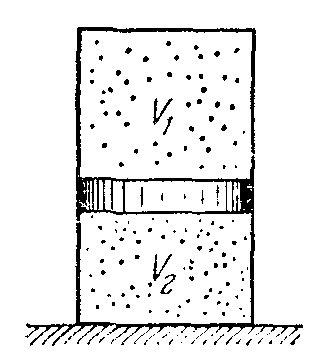
\includegraphics[scale=0.25]{0805GasLawsPiston.jpg}
\end{wrapfigure}

\AddProb В вертикальном закрытом сосуде имеется поршень, который может перемещаться без трения. 
По обе стороны от поршня находятся одинаковые массы одного и того же газа. 
При температуре $T$ объем верхней части в $n$ раз больше, чем объем нижней. 
Каким будет соотношение этих объемов, если повысить температуру до значения $T_2$?


\section{Молекулярно-кинетическая теория}

\begin{wrapfigure}{r}{5cm}
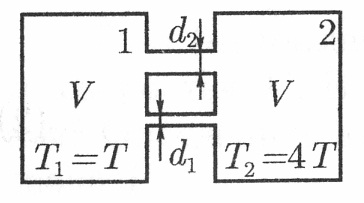
\includegraphics[scale=0.5]{0806KineticTheoryTwoVessels.jpg}
\end{wrapfigure}

%6
\AddProb Два сосуда одинакового объема соединены трубками. Диаметр одной из трубок велик, 
а другой мал по сравнению со средней длиной свободного пробега молекул газа, находящегося в сосуде. 
Первый сосуд поддерживается при температуре $T$, а второй при температуре $4T$. 
В каком направлении будет перетекать газ по узкой трубке, если перекрыть широкую трубку? 
Какая масса газа перейдет при этом из одного сосуд в другой, если общая масса газа в обоих сосудах равна $M$?

\begin{wrapfigure}{r}{3.2cm}
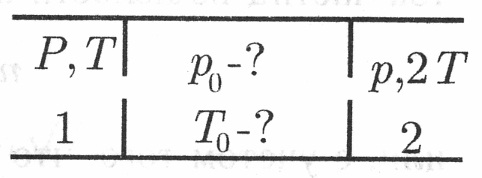
\includegraphics[scale=0.25]{0807KineticTheoryHelium.jpg}
\end{wrapfigure}

\AddProb Теплоизолированная полость небольшими малыми одинаковыми отверстиями соединена с двумя объемами, содержащими газообразный гелий. 
Давления в этих объемах поддерживаются одинаковыми и равными $P$, а температуры поддерживаются равными в одном из объемов $T$, в другом $2T$. 
Найдите установившиеся давление и температуру внутри полости.

\AddProb Плоская поверхность нагрета неравномерно, так что вдоль нее поддерживается градиент температуры $dT/dx$. 
В этих условиях газ, примыкающий к поверхности, приходит в движение вдоль поверхности. Это явление называют тепловым скольжением. 
Объясните его механизм и оцените скорость теплового скольжения. Необходимые параметры считать известными.

\AddProb (2008) Оценить по порядку величины установившуюся скорость, с которой будет двигаться в сильно разреженном воздухе плоский диск, 
одна из сторон которого нагрета до температуры $T_1$, а другая до температуры $T_2$, $T_1>T_2$. Температура воздуха равна $T$.

\AddProb (2009) Каково должно быть максимальное значение температурного градиента $dT/dz$ атмосферного воздуха, 
чтобы он мог находиться в устойчивом механическом равновесии? Воздух считать двухатомным газом с относительной молекулярной массой $\mu$. 
Ускорение свободного падения $g$ не зависит от высоты над поверхностью земли.